\documentclass[twoside]{book}

% Packages required by doxygen
\usepackage{fixltx2e}
\usepackage{calc}
\usepackage{doxygen}
\usepackage[export]{adjustbox} % also loads graphicx
\usepackage{graphicx}
\usepackage[utf8]{inputenc}
\usepackage{makeidx}
\usepackage{multicol}
\usepackage{multirow}
\PassOptionsToPackage{warn}{textcomp}
\usepackage{textcomp}
\usepackage[nointegrals]{wasysym}
\usepackage[table]{xcolor}

% Font selection
\usepackage[T1]{fontenc}
\usepackage[scaled=.90]{helvet}
\usepackage{courier}
\usepackage{amssymb}
\usepackage{sectsty}
\renewcommand{\familydefault}{\sfdefault}
\allsectionsfont{%
  \fontseries{bc}\selectfont%
  \color{darkgray}%
}
\renewcommand{\DoxyLabelFont}{%
  \fontseries{bc}\selectfont%
  \color{darkgray}%
}
\newcommand{\+}{\discretionary{\mbox{\scriptsize$\hookleftarrow$}}{}{}}

% Page & text layout
\usepackage{geometry}
\geometry{%
  a4paper,%
  top=2.5cm,%
  bottom=2.5cm,%
  left=2.5cm,%
  right=2.5cm%
}
\tolerance=750
\hfuzz=15pt
\hbadness=750
\setlength{\emergencystretch}{15pt}
\setlength{\parindent}{0cm}
\setlength{\parskip}{3ex plus 2ex minus 2ex}
\makeatletter
\renewcommand{\paragraph}{%
  \@startsection{paragraph}{4}{0ex}{-1.0ex}{1.0ex}{%
    \normalfont\normalsize\bfseries\SS@parafont%
  }%
}
\renewcommand{\subparagraph}{%
  \@startsection{subparagraph}{5}{0ex}{-1.0ex}{1.0ex}{%
    \normalfont\normalsize\bfseries\SS@subparafont%
  }%
}
\makeatother

% Headers & footers
\usepackage{fancyhdr}
\pagestyle{fancyplain}
\fancyhead[LE]{\fancyplain{}{\bfseries\thepage}}
\fancyhead[CE]{\fancyplain{}{}}
\fancyhead[RE]{\fancyplain{}{\bfseries\leftmark}}
\fancyhead[LO]{\fancyplain{}{\bfseries\rightmark}}
\fancyhead[CO]{\fancyplain{}{}}
\fancyhead[RO]{\fancyplain{}{\bfseries\thepage}}
\fancyfoot[LE]{\fancyplain{}{}}
\fancyfoot[CE]{\fancyplain{}{}}
\fancyfoot[RE]{\fancyplain{}{\bfseries\scriptsize Generated by Doxygen }}
\fancyfoot[LO]{\fancyplain{}{\bfseries\scriptsize Generated by Doxygen }}
\fancyfoot[CO]{\fancyplain{}{}}
\fancyfoot[RO]{\fancyplain{}{}}
\renewcommand{\footrulewidth}{0.4pt}
\renewcommand{\chaptermark}[1]{%
  \markboth{#1}{}%
}
\renewcommand{\sectionmark}[1]{%
  \markright{\thesection\ #1}%
}

% Indices & bibliography
\usepackage{natbib}
\usepackage[titles]{tocloft}
\setcounter{tocdepth}{3}
\setcounter{secnumdepth}{5}
\makeindex

% Hyperlinks (required, but should be loaded last)
\usepackage{ifpdf}
\ifpdf
  \usepackage[pdftex,pagebackref=true]{hyperref}
\else
  \usepackage[ps2pdf,pagebackref=true]{hyperref}
\fi
\hypersetup{%
  colorlinks=true,%
  linkcolor=blue,%
  citecolor=blue,%
  unicode%
}

% Custom commands
\newcommand{\clearemptydoublepage}{%
  \newpage{\pagestyle{empty}\cleardoublepage}%
}

\usepackage{caption}
\captionsetup{labelsep=space,justification=centering,font={bf},singlelinecheck=off,skip=4pt,position=top}

%===== C O N T E N T S =====

\begin{document}

% Titlepage & ToC
\hypersetup{pageanchor=false,
             bookmarksnumbered=true,
             pdfencoding=unicode
            }
\pagenumbering{alph}
\begin{titlepage}
\vspace*{7cm}
\begin{center}%
{\Large My Project }\\
\vspace*{1cm}
{\large Generated by Doxygen 1.8.13}\\
\end{center}
\end{titlepage}
\clearemptydoublepage
\pagenumbering{roman}
\tableofcontents
\clearemptydoublepage
\pagenumbering{arabic}
\hypersetup{pageanchor=true}

%--- Begin generated contents ---
\chapter{Hierarchical Index}
\section{Class Hierarchy}
This inheritance list is sorted roughly, but not completely, alphabetically\+:\begin{DoxyCompactList}
\item \contentsline{section}{Aquarium}{\pageref{classAquarium}}{}
\item \contentsline{section}{Entity}{\pageref{classEntity}}{}
\begin{DoxyCompactList}
\item \contentsline{section}{Coin}{\pageref{classCoin}}{}
\item \contentsline{section}{Food}{\pageref{classFood}}{}
\item \contentsline{section}{Guppy}{\pageref{classGuppy}}{}
\item \contentsline{section}{Piranha}{\pageref{classPiranha}}{}
\item \contentsline{section}{Snail}{\pageref{classSnail}}{}
\end{DoxyCompactList}
\item \contentsline{section}{Fish}{\pageref{classFish}}{}
\begin{DoxyCompactList}
\item \contentsline{section}{Guppy}{\pageref{classGuppy}}{}
\item \contentsline{section}{Piranha}{\pageref{classPiranha}}{}
\end{DoxyCompactList}
\item \contentsline{section}{Linked\+List$<$ T $>$}{\pageref{classLinkedList}}{}
\item \contentsline{section}{Linked\+List$<$ Coin $>$}{\pageref{classLinkedList}}{}
\item \contentsline{section}{Linked\+List$<$ Fish $>$}{\pageref{classLinkedList}}{}
\item \contentsline{section}{Linked\+List$<$ Food $>$}{\pageref{classLinkedList}}{}
\item \contentsline{section}{node$<$ T $>$}{\pageref{structnode}}{}
\item \contentsline{section}{node$<$ Coin $>$}{\pageref{structnode}}{}
\item \contentsline{section}{node$<$ Fish $>$}{\pageref{structnode}}{}
\item \contentsline{section}{node$<$ Food $>$}{\pageref{structnode}}{}
\item \contentsline{section}{Point}{\pageref{classPoint}}{}
\end{DoxyCompactList}

\chapter{Class Index}
\section{Class List}
Here are the classes, structs, unions and interfaces with brief descriptions\+:\begin{DoxyCompactList}
\item\contentsline{section}{\hyperlink{classAquarium}{Aquarium} }{\pageref{classAquarium}}{}
\item\contentsline{section}{\hyperlink{classCell}{Cell} }{\pageref{classCell}}{}
\item\contentsline{section}{\hyperlink{classCoin}{Coin} }{\pageref{classCoin}}{}
\item\contentsline{section}{\hyperlink{classEntity}{Entity} }{\pageref{classEntity}}{}
\item\contentsline{section}{\hyperlink{classFish}{Fish} }{\pageref{classFish}}{}
\item\contentsline{section}{\hyperlink{classFood}{Food} }{\pageref{classFood}}{}
\item\contentsline{section}{\hyperlink{classGuppy}{Guppy} }{\pageref{classGuppy}}{}
\item\contentsline{section}{\hyperlink{classLinkedList}{Linked\+List$<$ T $>$} }{\pageref{classLinkedList}}{}
\item\contentsline{section}{\hyperlink{structnode}{node$<$ T $>$} }{\pageref{structnode}}{}
\item\contentsline{section}{\hyperlink{classPiranha}{Piranha} }{\pageref{classPiranha}}{}
\item\contentsline{section}{\hyperlink{classPoint}{Point} }{\pageref{classPoint}}{}
\item\contentsline{section}{\hyperlink{classSnail}{Snail} }{\pageref{classSnail}}{}
\end{DoxyCompactList}

\chapter{Class Documentation}
\hypertarget{classAquarium}{}\section{Aquarium Class Reference}
\label{classAquarium}\index{Aquarium@{Aquarium}}


{\ttfamily \#include $<$Aquarium.\+hpp$>$}

\subsection*{Public Member Functions}
\begin{DoxyCompactItemize}
\item 
\mbox{\Hypertarget{classAquarium_aa1389622ce9474dbdc955e04b6efd1dc}\label{classAquarium_aa1389622ce9474dbdc955e04b6efd1dc}} 
{\footnotesize template$<$class T $>$ }\\T \hyperlink{classAquarium_aa1389622ce9474dbdc955e04b6efd1dc}{get\+Closest\+Entity} (T)
\begin{DoxyCompactList}\small\item\em Method untuk mendapatkan suatu entitas tertentu dengan jarak terdekat dari objek. \end{DoxyCompactList}\end{DoxyCompactItemize}


\subsection{Detailed Description}
Kelas yang merepresentasikan Akuarium dalam bentuk matriks 2D. Kelas ini akan menyimpan list yang berisi seluruh komponen yang ada di dalam akuarium. 

The documentation for this class was generated from the following file\+:\begin{DoxyCompactItemize}
\item 
Aquarium.\+hpp\end{DoxyCompactItemize}

\hypertarget{classCell}{}\section{Cell Class Reference}
\label{classCell}\index{Cell@{Cell}}


The documentation for this class was generated from the following file\+:\begin{DoxyCompactItemize}
\item 
Cell.\+hpp\end{DoxyCompactItemize}

\hypertarget{classCoin}{}\section{Coin Class Reference}
\label{classCoin}\index{Coin@{Coin}}


{\ttfamily \#include $<$Coin.\+hpp$>$}



Inheritance diagram for Coin\+:\nopagebreak
\begin{figure}[H]
\begin{center}
\leavevmode
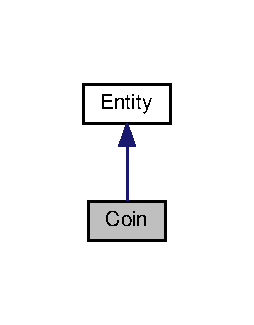
\includegraphics[width=122pt]{classCoin__inherit__graph}
\end{center}
\end{figure}


Collaboration diagram for Coin\+:\nopagebreak
\begin{figure}[H]
\begin{center}
\leavevmode
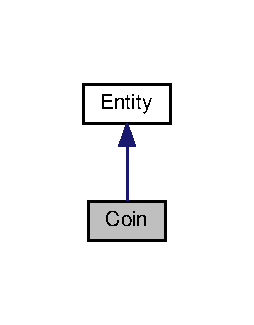
\includegraphics[width=122pt]{classCoin__coll__graph}
\end{center}
\end{figure}
\subsection*{Public Member Functions}
\begin{DoxyCompactItemize}
\item 
\mbox{\Hypertarget{classCoin_a94b2130e2d3ac956ba47271ad81c64f5}\label{classCoin_a94b2130e2d3ac956ba47271ad81c64f5}} 
\hyperlink{classCoin_a94b2130e2d3ac956ba47271ad81c64f5}{Coin} ()
\begin{DoxyCompactList}\small\item\em default ctor \end{DoxyCompactList}\item 
\mbox{\Hypertarget{classCoin_aa6bd6ccd1fe41c519112b077e54a603a}\label{classCoin_aa6bd6ccd1fe41c519112b077e54a603a}} 
\hyperlink{classCoin_aa6bd6ccd1fe41c519112b077e54a603a}{Coin} (int)
\begin{DoxyCompactList}\small\item\em ctor dengan paramater \end{DoxyCompactList}\item 
\mbox{\Hypertarget{classCoin_a1e51e734f8cbd7366e4376d9e3439d9e}\label{classCoin_a1e51e734f8cbd7366e4376d9e3439d9e}} 
int \hyperlink{classCoin_a1e51e734f8cbd7366e4376d9e3439d9e}{get\+Value} ()
\begin{DoxyCompactList}\small\item\em getter nilai value koin \end{DoxyCompactList}\item 
\mbox{\Hypertarget{classCoin_a000679bc7222f8ee0c0be74e920005a1}\label{classCoin_a000679bc7222f8ee0c0be74e920005a1}} 
void \hyperlink{classCoin_a000679bc7222f8ee0c0be74e920005a1}{set\+Value} (int)
\begin{DoxyCompactList}\small\item\em setter value pada koin \end{DoxyCompactList}\item 
\mbox{\Hypertarget{classCoin_a152d094662ff9b2ed44af94f11241856}\label{classCoin_a152d094662ff9b2ed44af94f11241856}} 
virtual void \hyperlink{classCoin_a152d094662ff9b2ed44af94f11241856}{move} ()
\begin{DoxyCompactList}\small\item\em method untuk koin bergerak \end{DoxyCompactList}\end{DoxyCompactItemize}


\subsection{Detailed Description}
Kelas \hyperlink{classCoin}{Coin} merupakan kelas turunan dari kelas \hyperlink{classEntity}{Entity} 

The documentation for this class was generated from the following file\+:\begin{DoxyCompactItemize}
\item 
Coin.\+hpp\end{DoxyCompactItemize}

\hypertarget{classEntity}{}\section{Entity Class Reference}
\label{classEntity}\index{Entity@{Entity}}


Inheritance diagram for Entity\+:
\nopagebreak
\begin{figure}[H]
\begin{center}
\leavevmode
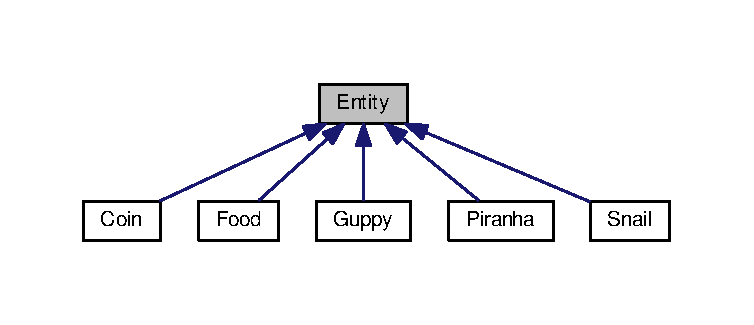
\includegraphics[width=350pt]{classEntity__inherit__graph}
\end{center}
\end{figure}
\subsection*{Public Member Functions}
\begin{DoxyCompactItemize}
\item 
\mbox{\Hypertarget{classEntity_a82c4f38635d70e83cbf17332e2abddc6}\label{classEntity_a82c4f38635d70e83cbf17332e2abddc6}} 
{\bfseries Entity} (int, int) \hyperlink{classPoint}{Point} get\+Position() const
\item 
\mbox{\Hypertarget{classEntity_ac8e667975506fcad1d4d3f0715c4df51}\label{classEntity_ac8e667975506fcad1d4d3f0715c4df51}} 
int {\bfseries get\+Velocity} () const
\item 
\mbox{\Hypertarget{classEntity_a1b9a6d2e14faa42afeea2b57218285fd}\label{classEntity_a1b9a6d2e14faa42afeea2b57218285fd}} 
void {\bfseries set\+Position} (\hyperlink{classPoint}{Point})
\item 
\mbox{\Hypertarget{classEntity_ab91bc74ca735bc2172d4eac1ed79ed2a}\label{classEntity_ab91bc74ca735bc2172d4eac1ed79ed2a}} 
void {\bfseries set\+Velocity} (int)
\item 
\mbox{\Hypertarget{classEntity_ac1f12a5f7922624ee7ced15be3b884de}\label{classEntity_ac1f12a5f7922624ee7ced15be3b884de}} 
void {\bfseries move} ()
\end{DoxyCompactItemize}


The documentation for this class was generated from the following file\+:\begin{DoxyCompactItemize}
\item 
Entity.\+hpp\end{DoxyCompactItemize}

\hypertarget{classFish}{}\section{Fish Class Reference}
\label{classFish}\index{Fish@{Fish}}


{\ttfamily \#include $<$Fish.\+hpp$>$}



Inheritance diagram for Fish\+:
\nopagebreak
\begin{figure}[H]
\begin{center}
\leavevmode
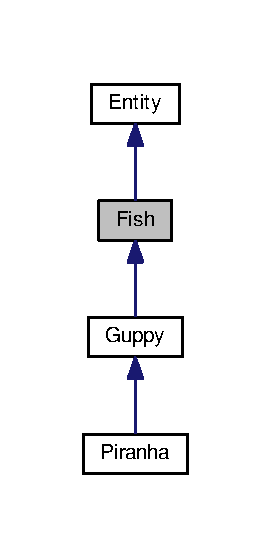
\includegraphics[width=130pt]{classFish__inherit__graph}
\end{center}
\end{figure}


Collaboration diagram for Fish\+:
\nopagebreak
\begin{figure}[H]
\begin{center}
\leavevmode
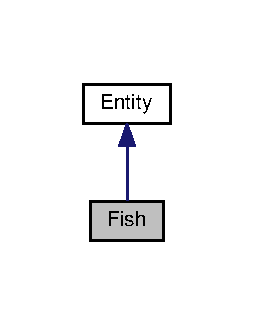
\includegraphics[width=122pt]{classFish__coll__graph}
\end{center}
\end{figure}
\subsection*{Public Member Functions}
\begin{DoxyCompactItemize}
\item 
\mbox{\Hypertarget{classFish_ab9c2e99efae1e293e660b02dfd6b3ec3}\label{classFish_ab9c2e99efae1e293e660b02dfd6b3ec3}} 
int \hyperlink{classFish_ab9c2e99efae1e293e660b02dfd6b3ec3}{get\+Fish\+State} () const
\begin{DoxyCompactList}\small\item\em Mendapatkan informasi tahap pertumbuhan dari suatu \hyperlink{classFish}{Fish}. \end{DoxyCompactList}\item 
\mbox{\Hypertarget{classFish_a6fec94dae5da20c2649e5cb4eab6288b}\label{classFish_a6fec94dae5da20c2649e5cb4eab6288b}} 
int \hyperlink{classFish_a6fec94dae5da20c2649e5cb4eab6288b}{get\+Foods\+To\+Grow} () const
\begin{DoxyCompactList}\small\item\em Mendapatkan informasi sejumlah makanan yang harus dimakan \hyperlink{classFish}{Fish} untuk memasuki tahap pertumbuhan selanjutnya. \end{DoxyCompactList}\item 
\mbox{\Hypertarget{classFish_aaeaf482b0fe949b02cd938dec4f4212d}\label{classFish_aaeaf482b0fe949b02cd938dec4f4212d}} 
int \hyperlink{classFish_aaeaf482b0fe949b02cd938dec4f4212d}{get\+Coin\+Time} () const
\begin{DoxyCompactList}\small\item\em Mendapatkan informasi waktu koin. \end{DoxyCompactList}\item 
\mbox{\Hypertarget{classFish_a111347fa2d2fb3ff52c697dd05ff2794}\label{classFish_a111347fa2d2fb3ff52c697dd05ff2794}} 
int \hyperlink{classFish_a111347fa2d2fb3ff52c697dd05ff2794}{get\+Coin\+Value} () const
\begin{DoxyCompactList}\small\item\em Mendapatkan informasi mengenai nilai koin yang dihasilkan suatu jenis \hyperlink{classFish}{Fish} tertentu. \end{DoxyCompactList}\item 
\mbox{\Hypertarget{classFish_a44f14e2464641108fde598d13021e58a}\label{classFish_a44f14e2464641108fde598d13021e58a}} 
int {\bfseries get\+Fish\+Value} () const
\item 
\mbox{\Hypertarget{classFish_afab92c9739af9d442b9e1623fb56a8d1}\label{classFish_afab92c9739af9d442b9e1623fb56a8d1}} 
bool \hyperlink{classFish_afab92c9739af9d442b9e1623fb56a8d1}{get\+Full} () const
\begin{DoxyCompactList}\small\item\em Mendapatkan informasi apakah \hyperlink{classFish}{Fish} dalam keadaan kenyang atau lapar. \end{DoxyCompactList}\item 
\mbox{\Hypertarget{classFish_aa2dfabcc7a6845d0bec12e77d234a269}\label{classFish_aa2dfabcc7a6845d0bec12e77d234a269}} 
bool \hyperlink{classFish_aa2dfabcc7a6845d0bec12e77d234a269}{get\+Right} () const
\begin{DoxyCompactList}\small\item\em Mendapatkan informasi apakah suatu \hyperlink{classFish}{Fish} menghadap ke kanan atau kiri. \end{DoxyCompactList}\item 
\mbox{\Hypertarget{classFish_a53f7a677495bf56d80d9d5aa00505e98}\label{classFish_a53f7a677495bf56d80d9d5aa00505e98}} 
void {\bfseries set\+Fish\+State} (int state)
\item 
\mbox{\Hypertarget{classFish_ac3f82829278b62ecc56fc68240b9a3f2}\label{classFish_ac3f82829278b62ecc56fc68240b9a3f2}} 
void {\bfseries set\+Foods\+To\+Grow} (int foods)
\item 
\mbox{\Hypertarget{classFish_a4283e7b3d67908fbf3c178a987159cb2}\label{classFish_a4283e7b3d67908fbf3c178a987159cb2}} 
void {\bfseries set\+Coin\+Time} (int c\+Time)
\item 
\mbox{\Hypertarget{classFish_ab61f43526d46c7edeee730be29c1eba0}\label{classFish_ab61f43526d46c7edeee730be29c1eba0}} 
void {\bfseries set\+Coin\+Value} (int value)
\item 
\mbox{\Hypertarget{classFish_af8633a8e349a04e3e1b4ee39e119b1e7}\label{classFish_af8633a8e349a04e3e1b4ee39e119b1e7}} 
void {\bfseries set\+Fish\+Value} (int value)
\item 
\mbox{\Hypertarget{classFish_aeb2dc6cb0b3e0b57a8e458824fdd1d5d}\label{classFish_aeb2dc6cb0b3e0b57a8e458824fdd1d5d}} 
void {\bfseries set\+Full} (bool)
\item 
\mbox{\Hypertarget{classFish_ad20d93cc7fdc5f560a06d120263feff6}\label{classFish_ad20d93cc7fdc5f560a06d120263feff6}} 
void {\bfseries set\+Right} (bool)
\end{DoxyCompactItemize}
\subsection*{Protected Member Functions}
\begin{DoxyCompactItemize}
\item 
\mbox{\Hypertarget{classFish_a45d7032d8c2eacedabb8a28799399adb}\label{classFish_a45d7032d8c2eacedabb8a28799399adb}} 
virtual void {\bfseries check\+Growth} ()=0
\item 
\mbox{\Hypertarget{classFish_acd7cbe8b09a544ca22e92a8edde1bacd}\label{classFish_acd7cbe8b09a544ca22e92a8edde1bacd}} 
virtual void {\bfseries spawn\+Coin} ()=0
\end{DoxyCompactItemize}
\subsection*{Protected Attributes}
\begin{DoxyCompactItemize}
\item 
\mbox{\Hypertarget{classFish_ab77f075818cbdd5e350379418a35172d}\label{classFish_ab77f075818cbdd5e350379418a35172d}} 
int {\bfseries state}
\item 
\mbox{\Hypertarget{classFish_a2a3e810d6b92aea2c29c69635c32a6ce}\label{classFish_a2a3e810d6b92aea2c29c69635c32a6ce}} 
int {\bfseries foods\+To\+Grow}
\item 
\mbox{\Hypertarget{classFish_ae9fdbf6d08fefff329bac0ee2e58ea2d}\label{classFish_ae9fdbf6d08fefff329bac0ee2e58ea2d}} 
int {\bfseries coin\+Time}
\item 
\mbox{\Hypertarget{classFish_a749b3925d3efc3a0b6278efccfe3dbea}\label{classFish_a749b3925d3efc3a0b6278efccfe3dbea}} 
int {\bfseries coin\+Value}
\item 
\mbox{\Hypertarget{classFish_acdd9042f3010004eb28bbd33fd215835}\label{classFish_acdd9042f3010004eb28bbd33fd215835}} 
int {\bfseries fish\+Value}
\item 
\mbox{\Hypertarget{classFish_af2e4a0561696f400efbb196c937f04cb}\label{classFish_af2e4a0561696f400efbb196c937f04cb}} 
bool {\bfseries is\+Full}
\item 
\mbox{\Hypertarget{classFish_a24723b3118965b94d4be7a48e31d482b}\label{classFish_a24723b3118965b94d4be7a48e31d482b}} 
bool {\bfseries is\+Right}
\end{DoxyCompactItemize}


\subsection{Detailed Description}
Kelas \hyperlink{classFish}{Fish} merupakan suatu kelas abstrak untuk objek fish Menangani seluruh method yang berlaku di seluruh kelas fish dan turunannya 

The documentation for this class was generated from the following files\+:\begin{DoxyCompactItemize}
\item 
Fish.\+hpp\item 
Fish.\+cpp\end{DoxyCompactItemize}

\hypertarget{classFood}{}\section{Food Class Reference}
\label{classFood}\index{Food@{Food}}


Inheritance diagram for Food\+:
\nopagebreak
\begin{figure}[H]
\begin{center}
\leavevmode
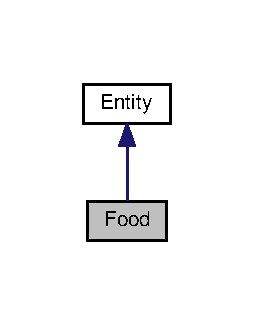
\includegraphics[width=122pt]{classFood__inherit__graph}
\end{center}
\end{figure}


Collaboration diagram for Food\+:
\nopagebreak
\begin{figure}[H]
\begin{center}
\leavevmode
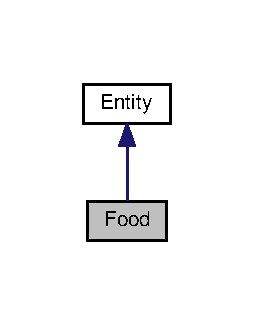
\includegraphics[width=122pt]{classFood__coll__graph}
\end{center}
\end{figure}
\subsection*{Public Member Functions}
\begin{DoxyCompactItemize}
\item 
\mbox{\Hypertarget{classFood_a342b2d30bd73b66d511aebd99ea3d0f9}\label{classFood_a342b2d30bd73b66d511aebd99ea3d0f9}} 
{\bfseries Food} (int, int)
\item 
\mbox{\Hypertarget{classFood_a8ab7250367a71b56cd52df3eb2eb0586}\label{classFood_a8ab7250367a71b56cd52df3eb2eb0586}} 
virtual void {\bfseries move} ()
\end{DoxyCompactItemize}


The documentation for this class was generated from the following file\+:\begin{DoxyCompactItemize}
\item 
Food.\+hpp\end{DoxyCompactItemize}

\hypertarget{classGuppy}{}\section{Guppy Class Reference}
\label{classGuppy}\index{Guppy@{Guppy}}


{\ttfamily \#include $<$Guppy.\+hpp$>$}



Inheritance diagram for Guppy\+:\nopagebreak
\begin{figure}[H]
\begin{center}
\leavevmode
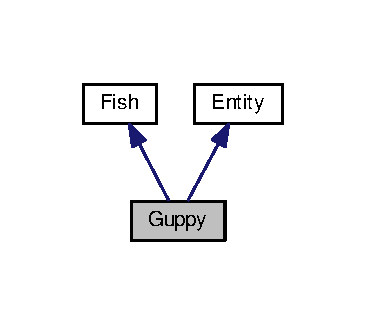
\includegraphics[width=176pt]{classGuppy__inherit__graph}
\end{center}
\end{figure}


Collaboration diagram for Guppy\+:\nopagebreak
\begin{figure}[H]
\begin{center}
\leavevmode
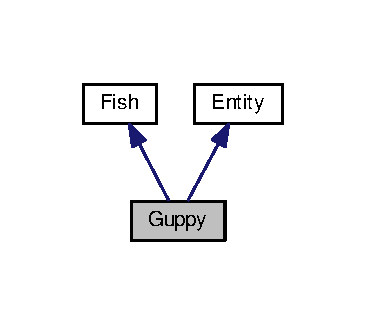
\includegraphics[width=176pt]{classGuppy__coll__graph}
\end{center}
\end{figure}
\subsection*{Public Member Functions}
\begin{DoxyCompactItemize}
\item 
\mbox{\Hypertarget{classGuppy_aa78f8b5323b1015c968a8edab52773f5}\label{classGuppy_aa78f8b5323b1015c968a8edab52773f5}} 
\hyperlink{classGuppy_aa78f8b5323b1015c968a8edab52773f5}{Guppy} ()
\begin{DoxyCompactList}\small\item\em default ctor \end{DoxyCompactList}\item 
\mbox{\Hypertarget{classGuppy_afe934262a0988e4ad041f4ed3a1a7e02}\label{classGuppy_afe934262a0988e4ad041f4ed3a1a7e02}} 
void \hyperlink{classGuppy_afe934262a0988e4ad041f4ed3a1a7e02}{eat} ()
\begin{DoxyCompactList}\small\item\em method untuk makan guppy \end{DoxyCompactList}\item 
\mbox{\Hypertarget{classGuppy_a06ceefb07ac8f6d590f8343c93c1edd9}\label{classGuppy_a06ceefb07ac8f6d590f8343c93c1edd9}} 
void \hyperlink{classGuppy_a06ceefb07ac8f6d590f8343c93c1edd9}{check\+Growth} ()
\begin{DoxyCompactList}\small\item\em method untuk mengetahui tahap pertumbuhan \hyperlink{classGuppy}{Guppy} \end{DoxyCompactList}\item 
\mbox{\Hypertarget{classGuppy_a58d97b8704a2635e7b7a1b365c37c570}\label{classGuppy_a58d97b8704a2635e7b7a1b365c37c570}} 
void \hyperlink{classGuppy_a58d97b8704a2635e7b7a1b365c37c570}{spawn\+Coin} ()
\begin{DoxyCompactList}\small\item\em method untuk menghasilkan koin \end{DoxyCompactList}\end{DoxyCompactItemize}
\subsection*{Additional Inherited Members}


\subsection{Detailed Description}
Kelas \hyperlink{classGuppy}{Guppy} merupakan kelas turunan dari \hyperlink{classFish}{Fish} dengan spesialisasi sifat-\/sifat \hyperlink{classGuppy}{Guppy} 

The documentation for this class was generated from the following file\+:\begin{DoxyCompactItemize}
\item 
Guppy.\+hpp\end{DoxyCompactItemize}

\hypertarget{classLinkedList}{}\section{Linked\+List$<$ T $>$ Class Template Reference}
\label{classLinkedList}\index{Linked\+List$<$ T $>$@{Linked\+List$<$ T $>$}}
\subsection*{Public Member Functions}
\begin{DoxyCompactItemize}
\item 
\mbox{\Hypertarget{classLinkedList_ac5a0d903d22d1157e98b6d3c182e1c74}\label{classLinkedList_ac5a0d903d22d1157e98b6d3c182e1c74}} 
bool {\bfseries Is\+Empty} ()
\item 
\mbox{\Hypertarget{classLinkedList_aad1e9d6d7611d4f0bfde0e90da2c108b}\label{classLinkedList_aad1e9d6d7611d4f0bfde0e90da2c108b}} 
void {\bfseries add} (T data)
\item 
\mbox{\Hypertarget{classLinkedList_a25079ed9b408efad63a1522c818d8705}\label{classLinkedList_a25079ed9b408efad63a1522c818d8705}} 
T {\bfseries get} (int index)
\item 
\mbox{\Hypertarget{classLinkedList_a35d443ed5be16bab9051c648e6e36d5e}\label{classLinkedList_a35d443ed5be16bab9051c648e6e36d5e}} 
int {\bfseries find} (T data)
\item 
\mbox{\Hypertarget{classLinkedList_ab9aa6e03f271785f6b488d8c4cc3f3c7}\label{classLinkedList_ab9aa6e03f271785f6b488d8c4cc3f3c7}} 
void {\bfseries remove} (T data)
\item 
\mbox{\Hypertarget{classLinkedList_a066a9a70c15be13a120b38305560135c}\label{classLinkedList_a066a9a70c15be13a120b38305560135c}} 
T {\bfseries operator\mbox{[}$\,$\mbox{]}} (int index)
\end{DoxyCompactItemize}
\subsection*{Public Attributes}
\begin{DoxyCompactItemize}
\item 
\mbox{\Hypertarget{classLinkedList_acaeb0499689a66aa0f0c6f71864da9a2}\label{classLinkedList_acaeb0499689a66aa0f0c6f71864da9a2}} 
\hyperlink{structnode}{node}$<$ T $>$ $\ast$ {\bfseries first}
\item 
\mbox{\Hypertarget{classLinkedList_ab584a6000168e8e43549dffda60240b2}\label{classLinkedList_ab584a6000168e8e43549dffda60240b2}} 
\hyperlink{structnode}{node}$<$ T $>$ $\ast$ {\bfseries last}
\end{DoxyCompactItemize}


The documentation for this class was generated from the following file\+:\begin{DoxyCompactItemize}
\item 
Linked\+List.\+hpp\end{DoxyCompactItemize}

\hypertarget{structnode}{}\section{node$<$ T $>$ Struct Template Reference}
\label{structnode}\index{node$<$ T $>$@{node$<$ T $>$}}


Collaboration diagram for node$<$ T $>$\+:\nopagebreak
\begin{figure}[H]
\begin{center}
\leavevmode
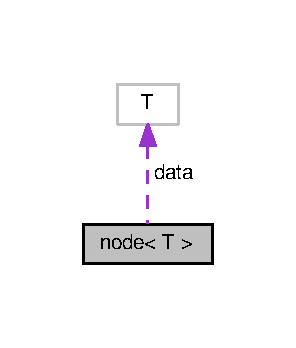
\includegraphics[width=142pt]{structnode__coll__graph}
\end{center}
\end{figure}
\subsection*{Public Attributes}
\begin{DoxyCompactItemize}
\item 
\mbox{\Hypertarget{structnode_ac96190e012822e6c053d2a5e9eedd68d}\label{structnode_ac96190e012822e6c053d2a5e9eedd68d}} 
\hyperlink{structnode}{node}$<$ T $>$ $\ast$ {\bfseries next}
\item 
\mbox{\Hypertarget{structnode_a0a3e961e5caf1562f0c27caef3940e7a}\label{structnode_a0a3e961e5caf1562f0c27caef3940e7a}} 
T {\bfseries data}
\end{DoxyCompactItemize}


The documentation for this struct was generated from the following file\+:\begin{DoxyCompactItemize}
\item 
Linked\+List.\+hpp\end{DoxyCompactItemize}

\hypertarget{classPiranha}{}\section{Piranha Class Reference}
\label{classPiranha}\index{Piranha@{Piranha}}


{\ttfamily \#include $<$Piranha.\+hpp$>$}



Inheritance diagram for Piranha\+:\nopagebreak
\begin{figure}[H]
\begin{center}
\leavevmode
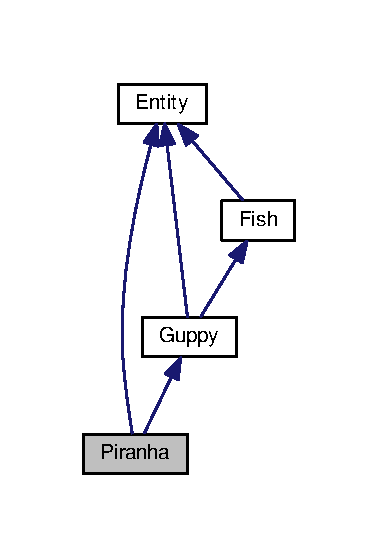
\includegraphics[width=182pt]{classPiranha__inherit__graph}
\end{center}
\end{figure}


Collaboration diagram for Piranha\+:\nopagebreak
\begin{figure}[H]
\begin{center}
\leavevmode
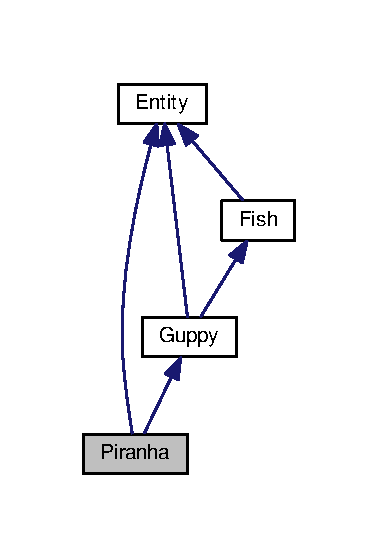
\includegraphics[width=182pt]{classPiranha__coll__graph}
\end{center}
\end{figure}
\subsection*{Public Member Functions}
\begin{DoxyCompactItemize}
\item 
\mbox{\Hypertarget{classPiranha_a7e3a4c5c7f458c16717c8cb997fc0331}\label{classPiranha_a7e3a4c5c7f458c16717c8cb997fc0331}} 
\hyperlink{classPiranha_a7e3a4c5c7f458c16717c8cb997fc0331}{Piranha} ()
\begin{DoxyCompactList}\small\item\em default ctor \end{DoxyCompactList}\item 
\mbox{\Hypertarget{classPiranha_ac48c0256edd56c427b3d82f6e0d4df82}\label{classPiranha_ac48c0256edd56c427b3d82f6e0d4df82}} 
void \hyperlink{classPiranha_ac48c0256edd56c427b3d82f6e0d4df82}{eat} ()
\begin{DoxyCompactList}\small\item\em method untuk makan \end{DoxyCompactList}\item 
\mbox{\Hypertarget{classPiranha_ad35beb897ca7281e3792faf8211e39a3}\label{classPiranha_ad35beb897ca7281e3792faf8211e39a3}} 
void \hyperlink{classPiranha_ad35beb897ca7281e3792faf8211e39a3}{check\+Growth} ()
\begin{DoxyCompactList}\small\item\em method untuk mengetahui tahap pertumbuhan \hyperlink{classPiranha}{Piranha} \end{DoxyCompactList}\item 
\mbox{\Hypertarget{classPiranha_ad17da28a5556a91170fb6bfe4e331b82}\label{classPiranha_ad17da28a5556a91170fb6bfe4e331b82}} 
void \hyperlink{classPiranha_ad17da28a5556a91170fb6bfe4e331b82}{spawn\+Coin} ()
\begin{DoxyCompactList}\small\item\em method untuk menghasilkan koin \end{DoxyCompactList}\end{DoxyCompactItemize}
\subsection*{Additional Inherited Members}


\subsection{Detailed Description}
Kelas \hyperlink{classPiranha}{Piranha} merupakan kelas turunan dari \hyperlink{classFish}{Fish} dengan spesialisasi sifat-\/sifat \hyperlink{classPiranha}{Piranha} 

The documentation for this class was generated from the following files\+:\begin{DoxyCompactItemize}
\item 
Piranha.\+hpp\item 
Piranha.\+cpp\end{DoxyCompactItemize}

\hypertarget{classPoint}{}\section{Point Class Reference}
\label{classPoint}\index{Point@{Point}}
\subsection*{Public Member Functions}
\begin{DoxyCompactItemize}
\item 
\mbox{\Hypertarget{classPoint_a7e2f39fba71990705aac9ffee1b389b4}\label{classPoint_a7e2f39fba71990705aac9ffee1b389b4}} 
{\bfseries Point} (int, int)
\item 
\mbox{\Hypertarget{classPoint_a5b7ec0fb127734c1cd5c6f350a3990fc}\label{classPoint_a5b7ec0fb127734c1cd5c6f350a3990fc}} 
{\bfseries Point} (const \hyperlink{classPoint}{Point} \&)
\item 
\mbox{\Hypertarget{classPoint_aecfc6968998d806384e24cd93072b024}\label{classPoint_aecfc6968998d806384e24cd93072b024}} 
\hyperlink{classPoint}{Point} \& {\bfseries operator=} (const \hyperlink{classPoint}{Point} \&)
\item 
\mbox{\Hypertarget{classPoint_ac9d5859db121c7d1b89ca89266dca0a3}\label{classPoint_ac9d5859db121c7d1b89ca89266dca0a3}} 
int {\bfseries getX} () const
\item 
\mbox{\Hypertarget{classPoint_a86d10ff46e08462c45b15a8c7ef62d61}\label{classPoint_a86d10ff46e08462c45b15a8c7ef62d61}} 
int {\bfseries getY} () const
\item 
\mbox{\Hypertarget{classPoint_a70df49e9bd07a4b86fd7c3fcb72b6fed}\label{classPoint_a70df49e9bd07a4b86fd7c3fcb72b6fed}} 
void {\bfseries setX} (int)
\item 
\mbox{\Hypertarget{classPoint_a00952d11c8b02ecf9d584b232edeee42}\label{classPoint_a00952d11c8b02ecf9d584b232edeee42}} 
void {\bfseries setY} (int)
\end{DoxyCompactItemize}


The documentation for this class was generated from the following file\+:\begin{DoxyCompactItemize}
\item 
Point.\+hpp\end{DoxyCompactItemize}

\hypertarget{classSnail}{}\section{Snail Class Reference}
\label{classSnail}\index{Snail@{Snail}}


Inheritance diagram for Snail\+:
\nopagebreak
\begin{figure}[H]
\begin{center}
\leavevmode
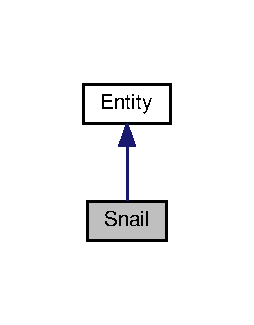
\includegraphics[width=122pt]{classSnail__inherit__graph}
\end{center}
\end{figure}


Collaboration diagram for Snail\+:
\nopagebreak
\begin{figure}[H]
\begin{center}
\leavevmode
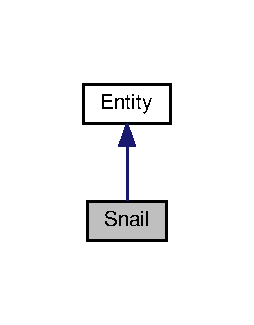
\includegraphics[width=122pt]{classSnail__coll__graph}
\end{center}
\end{figure}
\subsection*{Public Member Functions}
\begin{DoxyCompactItemize}
\item 
\mbox{\Hypertarget{classSnail_a47d29cb68815627114634e5f5739a591}\label{classSnail_a47d29cb68815627114634e5f5739a591}} 
virtual void {\bfseries move} ()
\end{DoxyCompactItemize}


The documentation for this class was generated from the following file\+:\begin{DoxyCompactItemize}
\item 
Snail.\+hpp\end{DoxyCompactItemize}

%--- End generated contents ---

% Index
\backmatter
\newpage
\phantomsection
\clearemptydoublepage
\addcontentsline{toc}{chapter}{Index}
\printindex

\end{document}
